\section{Experiments}

\subsection{Setup}
We conducted our experiments on three benchmarks, Webkb, ER and Protein, all of which are publicly available in Alchemy~\cite{kok&al06}. Further, we created a new dataset from Yelp reviews, and analyzed our approach with this dataset. We implemented Obj2Vec using the Gensim package~\cite{rehurek_lrec}.

\eat{
We first took 5$\%$ subsets of each benchmark which we consider as gold standard and refer as GS since original data cannot be run in the state-of-the-art MLN systems e.g. Tuffy~\cite{niu&al11} and Magician~\cite{magician16} which implements scalable versions of contrastive divergence (CD), voted perceptron (VP) and pseudo-log-likelihood maximisation (PLL), using approximate counting oracles~\cite{sarkhel&al16}. We generated compressed distribution of benchmarks using our neural embedding approach which we refer as NE, generated another compressed distribution using  another baseline method where we used Venugopal and Gogate's~\cite{venugopal&gogate14} approach (available in the Magician open-source code) and refer as VG. We generated another compressed distribution sampling evidence atoms randomly and refer to this as Random. So, each meta atom from compressed distributions represents multiple atoms of GS. We ran marginal inference on compressed datasets and GS in Magician which is available as open-source.
}

We compared our Obj2Vec-based lifting approach which we refer to as NE, with Venugopal and Gogate's~\cite{venugopal&gogate14} approach (VG) available in Magician~\cite{magician16}, where they compress the MLN using K-Means clustering, using features based on counts of formulas satisfied by the evidence. To make the comparison fair, we ensured that we reduced each domain to 10$\%$ of its original value in both NE as well as VG. For our Obj2vec architecture, we set the number of number of neurons in the hidden layer as $10\%$ of the total number of objects in the MLN. For a sanity check, we also added an alternative approach, which we refer to as Random, where we sample evidence atoms randomly to reduce the size of the MLN.

\eat{
We got marginal probabilities for query meta atoms while we ran marginal inference on compressed distributions and compared the resulting marginals with marginals of GS. We used a threshold value to determine atoms as true or false. Since each meta atom from compressed distribution represents multiple atoms of GS, we treated those atoms as true if that meta atom is true from marginal inference output and false if the meta atom is false and compared the marginal inference results of compressed distributions to GS and computed F-measure.
}

\eat{
We also experimented NE on review spam benchmark from Yelp where each review having a score is written by a user for a restaurant and each review contains some word which we represented by a simple MLN : ${\tt R}$ (review) $\wedge$ ${\tt S}$ (review,word) $\wedge$ ${\tt T}$ (review,user) $\wedge$ ${\tt U}$ (review,restaurant) $\wedge$ ${\tt V}$ (review,score). Then we applied our NE on this MLN with the purpose that symmetric reviews should have similar restaurants and users as NE considers joint dependency among domains.
}

\subsection{Results}

\eat{
We evaluated our approach on three key aspects, (i) Solution Assurance, (ii) Solution Quality, and, (iii) Scalability. To ensure that our idea is promising, we have created a synthetic benchmark where symmetry among domain objects can be easily detected and reported how  accurately our approach finds symmetries among objects as we increase number of formulas in MLN. For quality, we have reported F-measure of NE, VG and Random and finally, we have reported running time of each approach to ensure the scalability.
}
We evaluate our approach on the accuracy of inference, ability to detect symmetries, and scalability.
\subsubsection{Accuracy}
\eat{
We compared marginal inference result for NE, VG and Random with GS and computed F-measure for the benchmarks. Fig.~\ref{fig:quality} exhibits that our NE significantly outperforms both VG and Random for all of the benchmarks. We applied NE on review spam benchmark and picked 10 top symmetric reviews and tried to plot similarity scores of those reviews and also similarity scores of the respective users and restaurants. As we described earlier, symmetric reviews supposed to have symmetric users and restaurants which is reflected in Table~\ref{tab:score} and the result affirms our claim that NE considers joint dependency across domains.
}
We first constructed a gold standard for query variables in our benchmarks as follows. For each of the benchmarks, we learned the weights using Magician~\cite{magician16}. We then used around $10\%$ of the benchmark as test data, to ensure that the inference results were obtained were reliable using existing inference methods. We used Magician to perform marginal inference on the benchmark. We then used a threshold to obtain the classification on the query variables of our benchmarks. We consider this result as gold-standard results (GS). We then applied NE and VG to the same test data, and compared the classification of query variables using NE and VG, with GS, in terms of the F1-score. Fig.~\ref{fig:quality} shows our results. Here, we see that NE significantly outperforms both VG and Random for all three of the benchmarks.

\begin{figure}
  \centering
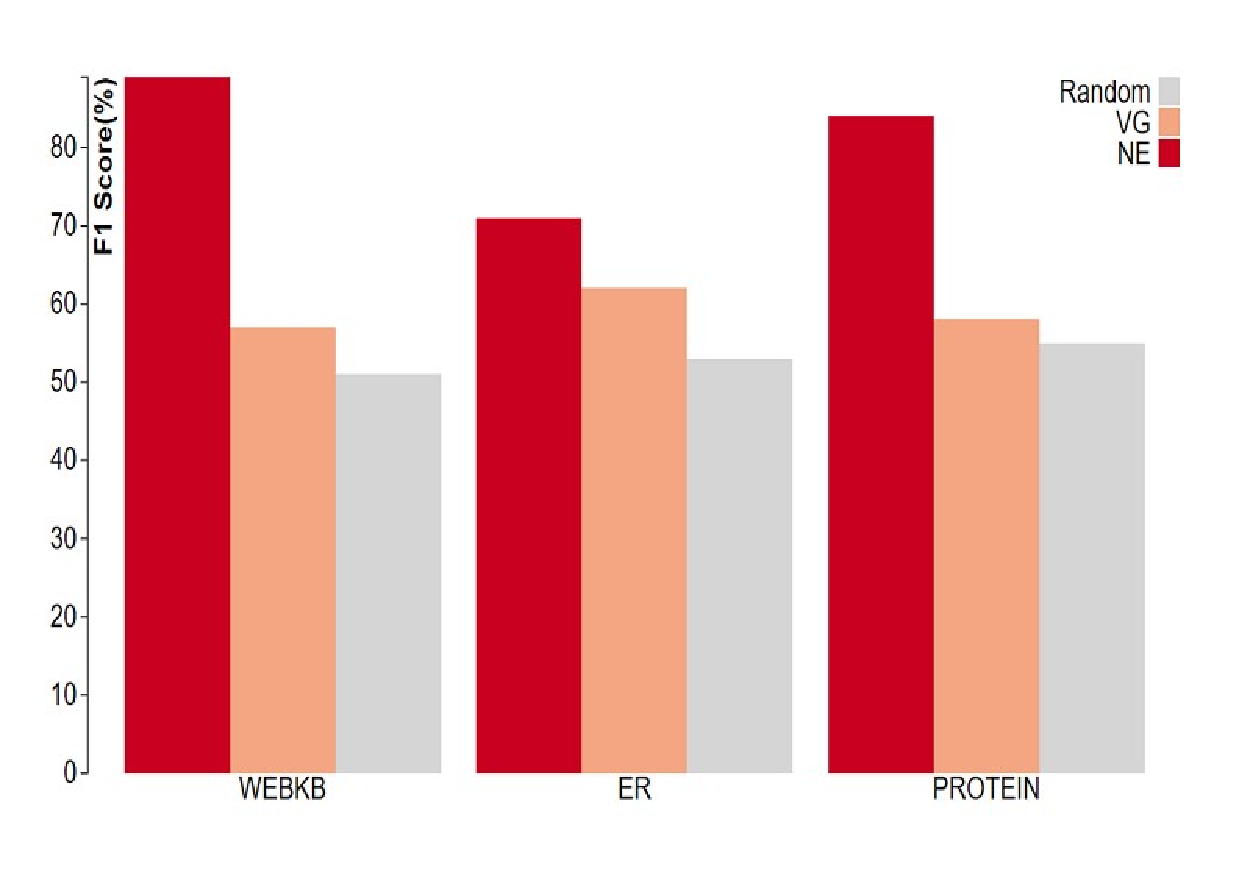
\includegraphics[scale=0.40]{quality.pdf}
\caption{\small{\label{fig:quality} Comparison of F-measures of approximate results on benchmarks using various approaches, as compared to the gold standard  (GS) results.}}
\end{figure}

\subsubsection{Symmetry Detection}

We evaluated the effect of increasing the context on symmetry detection. Specifically, we considered a simple synthetic MLN, where we incrementally add formulas of the form ${\tt R}(x)$ $\wedge$ ${\tt P}_i(x,y)$. Initially, we have a single formula, and add  evidences such that there is a common context for specific objects in $\Delta_x$. Our aim is to detect all those objects of $\Delta_x$ as being symmetric to each other. As we add more formulas, the common context for the symmetric objects in $\Delta_x$ keeps increasing. Fig.~\ref{fig:symmetry} shows our results in terms of the $\%$ of symmetric objects we could detect as we increase the number of formulas, i.e., as we add ${\tt R}(x)$ $\wedge$ ${\tt P}_1(x,y)$, ${\tt R}(x)$ $\wedge$ ${\tt P}_2(x,y)$, etc. Our results clearly shows that as the amount of context for symmetric objects in $\Delta_x$ increases, symmetry detection becomes more accurate.

%To do this, for every object, we obtained the list of similar objects in the embedding, and considered these as symmetric objects
\begin{figure}
  \centering
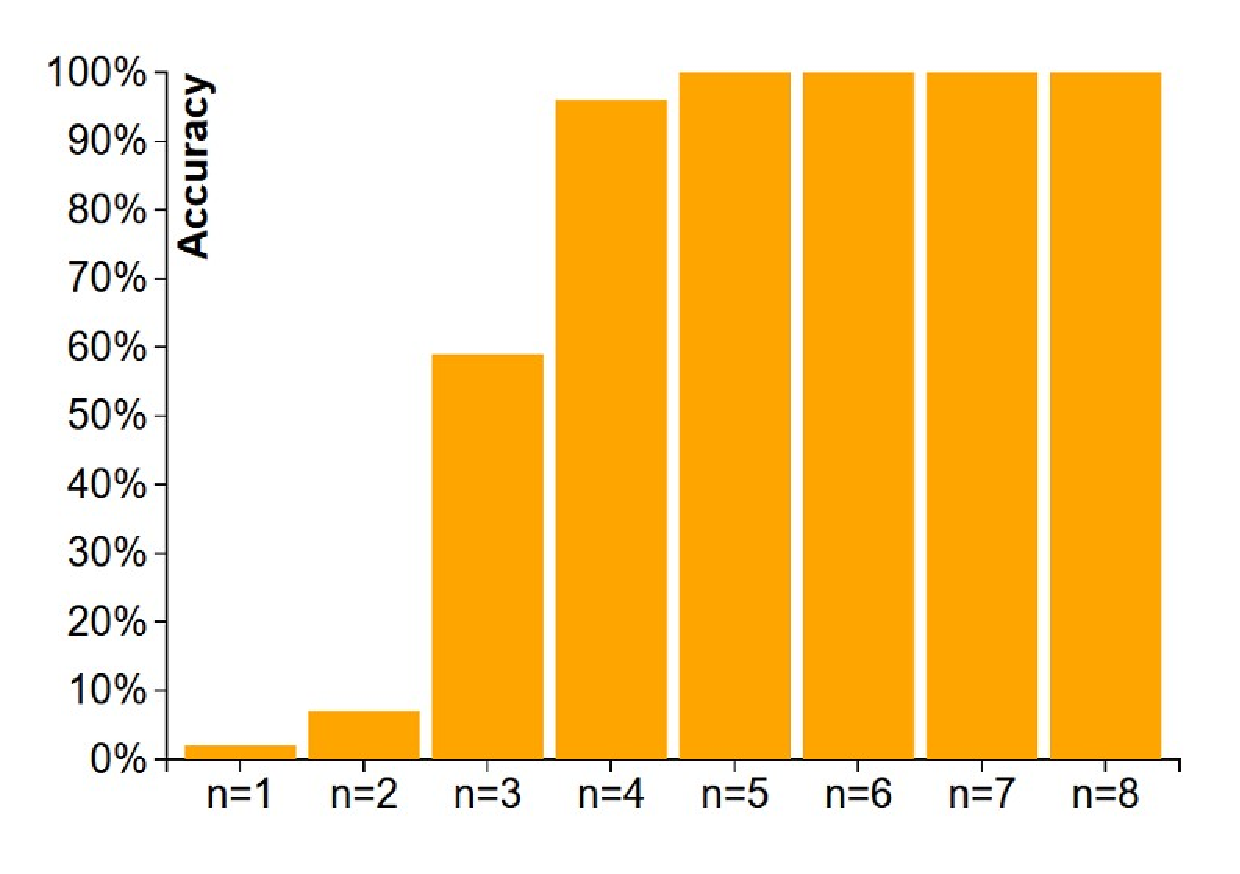
\includegraphics[scale=0.40]{symmetry.pdf}
\caption{\small{\label{fig:symmetry} Accuracy in detecting symmetries as we increase the context.}}
\end{figure} 

Next, we considered the effect of joint dependencies among multiple domains. Specifically, we analyzed the correlation between the symmetry of one domain and the symmetry of other, related domains. For this, we used a real-world dataset consisting of reviews from Yelp. Specifically, we used 7000 reviews written by around 200 users regarding around 800 restaurants.  Each review had a score (between 1 and 5) given by a user, and each review was written for a specific restaurant. For our experiment, we considered a simple MLN structure: ${\tt Word}$ ($review$,$word$) $\wedge$ ${\tt User}$ ($review$, $user$) $\wedge$ ${\tt Rest}$ ($review$, $restaurant$) $\Rightarrow$ ${\tt Score}$ ($review$, $score$). We embed the domain objects using Obj2vec, and then for each review $R$, we computed $k$ of its closest neighbors in the embedding. For each of $R$'s neighbors, we computed the similarity between the review vectors, the similarity between user vectors corresponding to users who wrote the reviews, and the similarity between restaurant vectors corresponding to restaurants about which the reviews were written. We then averaged these similarity values over all reviews over varying values of $k$ (between 1 to 10). As shown by the results in Fig~\ref{tab:score}, symmetries in the reviews, closely correlates to symmetries on the user who wrote the reviews, and symmetries on the restaurants for which the review was written. As our neighborhood size increases, the similarity scores go down uniformly. Thus, each variable's symmetry has a dependency upon the other variables.

%Then we applied our NE on this MLN with the purpose that symmetric reviews should have similar restaurants and users as NE considers joint dependency among domains.


\eat{
To ascertain our claim, we created an arbitrary MLN having $f_1$ $\ldots$ $f_n$ formulas of the form ${\tt R}(x)$ $\wedge$ ${\tt S}(x,y)$. Then we added symmetric evidence atoms like ${\tt R}(x_i)$,${\tt S}(x_i,y_j)$ where ${\tt i}$ $\%$ ${\tt k}$  = ${\tt j}$ for any constant ${\tt k}$. We added symmetric atom this way to test whether our NE can identify the symmetry. We noticed that NE accuracy increases as we increase number of formulas. Fig.~\ref{fig:symmetry} shows that accuracy becomes 100$\%$ for ${\tt n}$=5.
}



 



\eat{
\begin{table}[]
  \centering
  \fontsize{20}{9}\selectfont
  \resizebox{0.47\textwidth}{!}{
 %\tabcolsep=0.15cm
\begin{tabular}{| c | c | c | c |}
\hline
\rule{0pt}{20pt}\textbf{Review} & \textbf{Review Score} & \textbf{User Score} & \textbf{Rest Score}\\[0ex]
\hline
\rule{0pt}{20pt}Review 1   &   0.73 & 0.86 & 0.99 \\[0ex]
\rule{0pt}{20pt}Review 3   &   0.72 & 0.96 & 0.99 \\[0ex]
\rule{0pt}{20pt}Review 3   &   0.70 & 0.98 & 0.99 \\[0ex]
\rule{0pt}{20pt}Review 4   &   0.67 & 0.91 & 0.99 \\[0ex]
\rule{0pt}{20pt}Review 5   &   0.66 & 0.88 & 0.98 \\[0ex]
\rule{0pt}{20pt}Review 6   &   0.66 & 0.98 & 0.99 \\[0ex]
\rule{0pt}{20pt}Review 7   &   0.63 & 0.98 & 0.99 \\[0ex]
\rule{0pt}{20pt}Review 8   &   0.60 & 0.97 & 0.99 \\[0ex]
\rule{0pt}{20pt}Review 9   &   0.60 & 0.76 & 0.99 \\[0ex]
\rule{0pt}{20pt}Review 10   &   0.60 & 0.94 & 0.99 \\[0ex]
\hline
\end{tabular}
  }
  \normalsize
  \caption {\label{tab:score}Comparison of similarity scores of top 10 reviews and their respective users and restaurants.}
\end{table}
}

\begin{table}[]
  \centering
  \fontsize{20}{9}\selectfont
  \resizebox{0.47\textwidth}{!}{
 %\tabcolsep=0.15cm
\begin{tabular}{| c | c | c | c |}
\hline
\rule{0pt}{20pt}\textbf{ Nearest reviews ($k$)} & \textbf{Avg Review Sim} & \textbf{Avg User Sim} & \textbf{Avg Rest Sim}\\[0ex]
\hline
\rule{0pt}{20pt} 1   &   1.00 & 0.99 & 1.00 \\[0ex]
\rule{0pt}{20pt} 2   &   0.73 & 0.99 & 0.99 \\[0ex]
\rule{0pt}{20pt} 3   &   0.70 & 0.91 & 0.89 \\[0ex]
\rule{0pt}{20pt} 4   &   0.60 & 0.71 & 0.78 \\[0ex]
\rule{0pt}{20pt} 5   &   0.59 & 0.71 & 0.78 \\[0ex]
\rule{0pt}{20pt} 6   &   0.58 & 0.72 & 0.78 \\[0ex]
\rule{0pt}{20pt} 7   &   0.57 & 0.68 & 0.71 \\[0ex]
\rule{0pt}{20pt} 8   &   0.55 & 0.72 & 0.68 \\[0ex]
\rule{0pt}{20pt} 9   &   0.51 & 0.7 & 0.72 \\[0ex]
\rule{0pt}{20pt} 10  &   0.50 & 0.67 & 0.71 \\[0ex]
\hline
\end{tabular}
  }
  \normalsize
  \caption {\label{tab:score}Average similarity score of reviews, users and restaurants as we increase number of nearest reviews.}
\end{table}

\subsubsection{Scalability}

\eat{
Fig.~\ref{fig:time} illustrates required time for compression and inference as our ultimate goal is to reduce time. Fig.~\ref{fig:time}, exhibits that our NE takes almost similar time compared to VG and Random while compression time for each approach is trivial but inference takes notably less time compared to GS which makes our approach scalable and practical.
 }
 We evaluate scalability of our approach in terms of time required to generate the embedding and reduce the objects, as well as time for inference on the reduced MLN. Fig.~\ref{fig:time} shows our results for time required to generate the reduced MLN. Here, NE takes slightly longer than VG for reducing the MLN on the WebKB and ER datasets, and is almost the same for the protein dataset. The inference time on the reduced MLN was nearly the same for both NE and VG.
\begin{figure}
  \centering
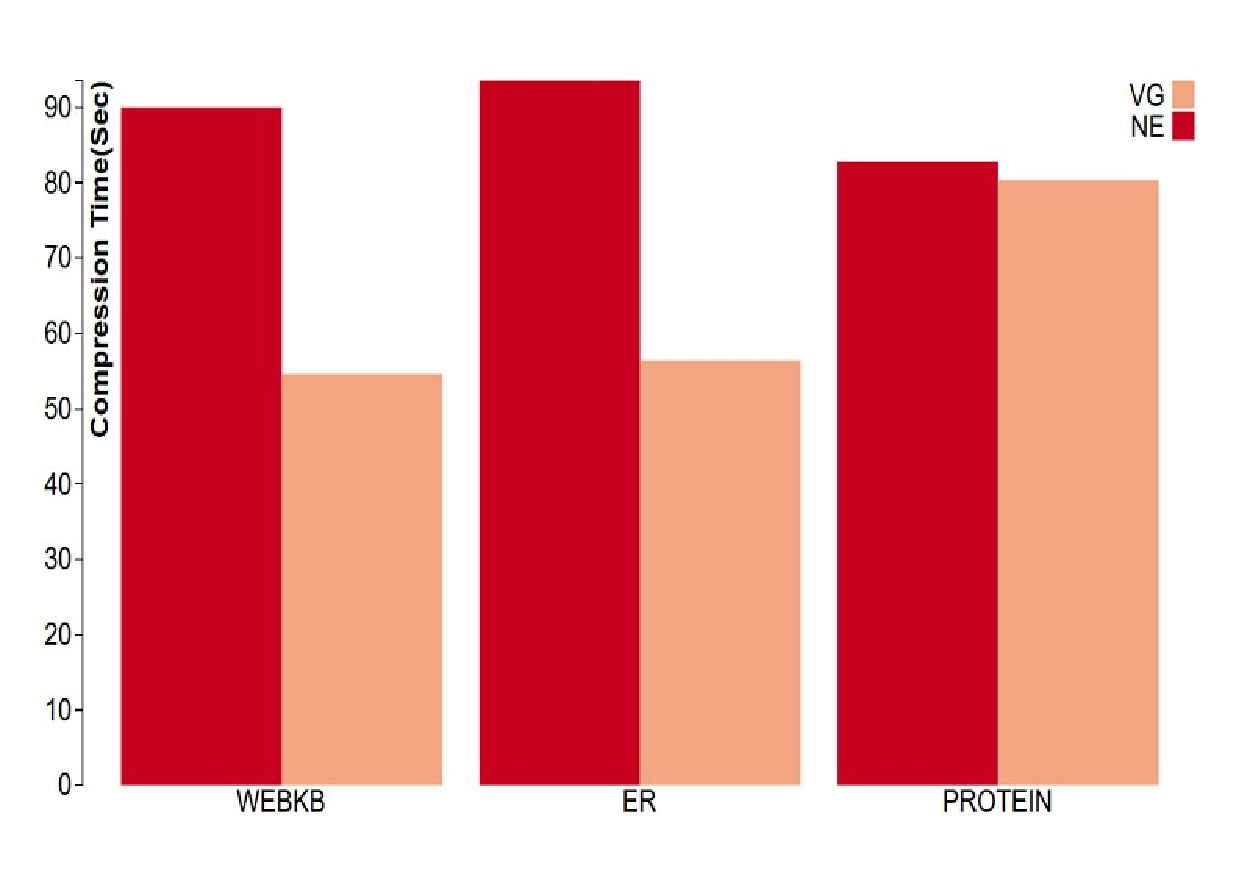
\includegraphics[scale=0.40]{compress_time.pdf}
\caption{\small{\label{fig:time} Comparison of running time for NE and VG.}}
\end{figure}

\eat{
\begin{figure}
  \centering
\includegraphics[scale=0.40]{inference.pdf}
\caption{\small{\label{fig:time} Comparison of compression and inference time for GS, NE, VG and Random.}}
\end{figure}
}